\documentclass{article}
\usepackage[utf8]{inputenc}
\usepackage[spanish]{babel}
\usepackage{listings}
\usepackage{graphicx}
\graphicspath{ {images/} }
\usepackage{cite}

\begin{document}

\begin{titlepage}
    \begin{center}
        \vspace*{1cm}
            
        \Huge
        \textbf{Planificación del Parcial 2}
            
        \vspace{0.5cm}
        \LARGE
            
        \vspace{1.5cm}
            
        \textbf{Juan Camilo Mazo Castro}\\
        \textbf{Santiago Pereira Ramirez}
            
        \vfill
            
        \vspace{0.8cm}
            
        \Large
        Despartamento de Ingeniería Electrónica y Telecomunicaciones\\
        Universidad de Antioquia\\
        Medellín\\
        Septiembre de 2021
            
    \end{center}
\end{titlepage}

\tableofcontents
\newpage
\section{Comprension del problema}\label{intro}
Se deberá a partir de una imagen de una bandera, representarla a través de una matriz de leds RGBs en el programa Tinkerkad y el entorno de desarrollo Qt creator\\

Se debe construir un algoritmo que permita escalar una imagen de tamaño nxn pixeles a el tamaño de la matriz de leds que construyamos.\\

\subsection{Elementos a emplear} \label{contenido}
Para la práctica se deberá de utilizar clases y objetos para el empleo de los algoritmos que se deben de utilizar y las demás funciones y métodos para el correcto empleo del programa, los valores que obtengamos de la imagen (con ayuda de de la librería QImage del entorno de Qtcreator) se podrán almacenar por medio de contenedores o matrices dinámicas, ya que estos requieren utilizar memoria dinámica.\\

Así mismo deberemos de trabajar con Arduino en la plataforma Tinkerkad, con elementos como tiras de Neopixel, suministro de energía para dar suficiente energía para la matriz de 20x20.\\

\subsection{Clases y relación} \label{contenido}

--Emplearemos una clase llamada talvez "ImageReSize" donde podremos escalar la imagen y obtener sus datos, ahora tendrán métodos por ejemplo para pedir el nombre de la imagen, también para mostrar la matriz de colores(RGB) redimensionada o el método que nos permitirá llevar los datos a archivo "Datos.txt".\\

\section{Programacion y tareas } \label{contenido}

--Hacer el archivo donde se planificará el desarrollo del parcial.

--Se creará el archivo de Qt y se deberá de hacer pruebas con los conocimientos acerca de la manipulación de imágenes, 
Después de esto se podrá construir la clase que nos permitirá crear los métodos de muestreo para redimensionar la imagen y llevar los datos hacia un documento.\\

--Empezar a crear el algoritmo de submuestreo y sobremuestreo, hacer las diversas pruebas para verificar que se este desarrollando de buena manera.\\

--crear el Tinkercad y escoger cual es el tamaño adecuado para la matriz de led RGBs.\\

--Hacer las diferentes conexiones con el arduino.\\

-- Crear un método que reciba los datos del método de muestreo.\\

--Utilizar la función para prender los leds RGBs en Arduino y copiar la información en él.\\

--Hacer pruebas con diferentes banderas, para tener certeza de que el programa funciona bien.\\

--Revisar los métodos del objeto.\\

--realizar el informe final.\\

--Grabar el video.\\

\section{Algoritmo Implementado}

Este algoritmo hace referencia a una media de datos. Saca un promedio de cierta cantidad de datos de pixeles, esto con el fin de escalar la imagen.\\

A continuación el seudocódigo se podrá ver en Figura 1 y figura 2:\\

\begin{figure}[h]
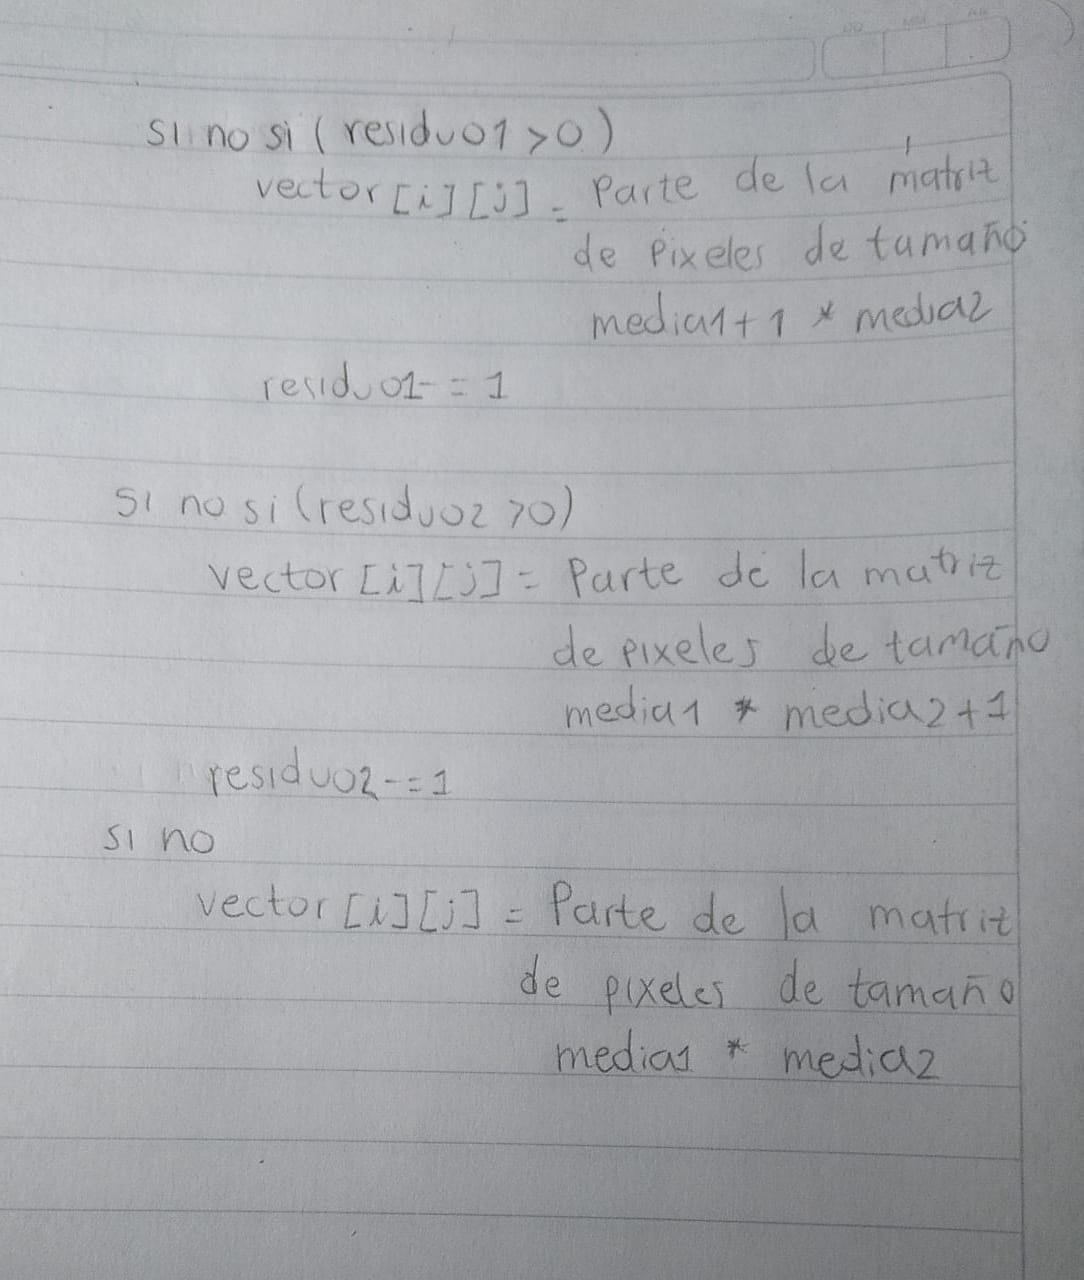
\includegraphics[width=8 cm]{Imagen_3.jpeg}
\centering
\caption{Pseudocódigo 1}
\label{fig:Imagen_4}
\end{figure}



\begin{figure}[h]
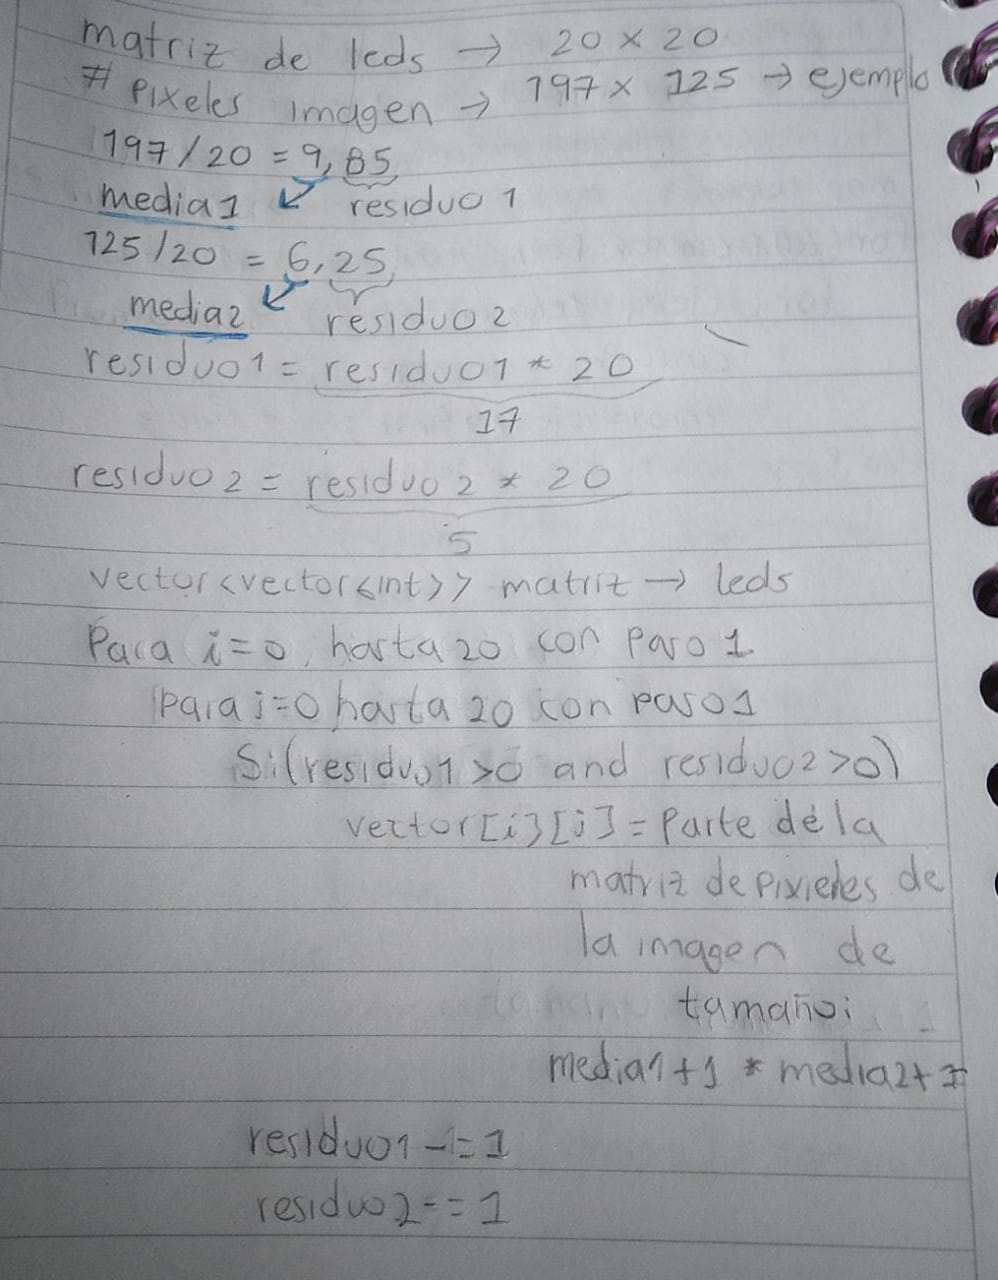
\includegraphics[width=8 cm]{Imagen_4.jpeg}
\centering
\caption{Pseudocódigo 2}
\label{fig:Imagen_4}
\end{figure}



Una representación visual se puede visualizar en figura 3:\\

\begin{figure}[h]
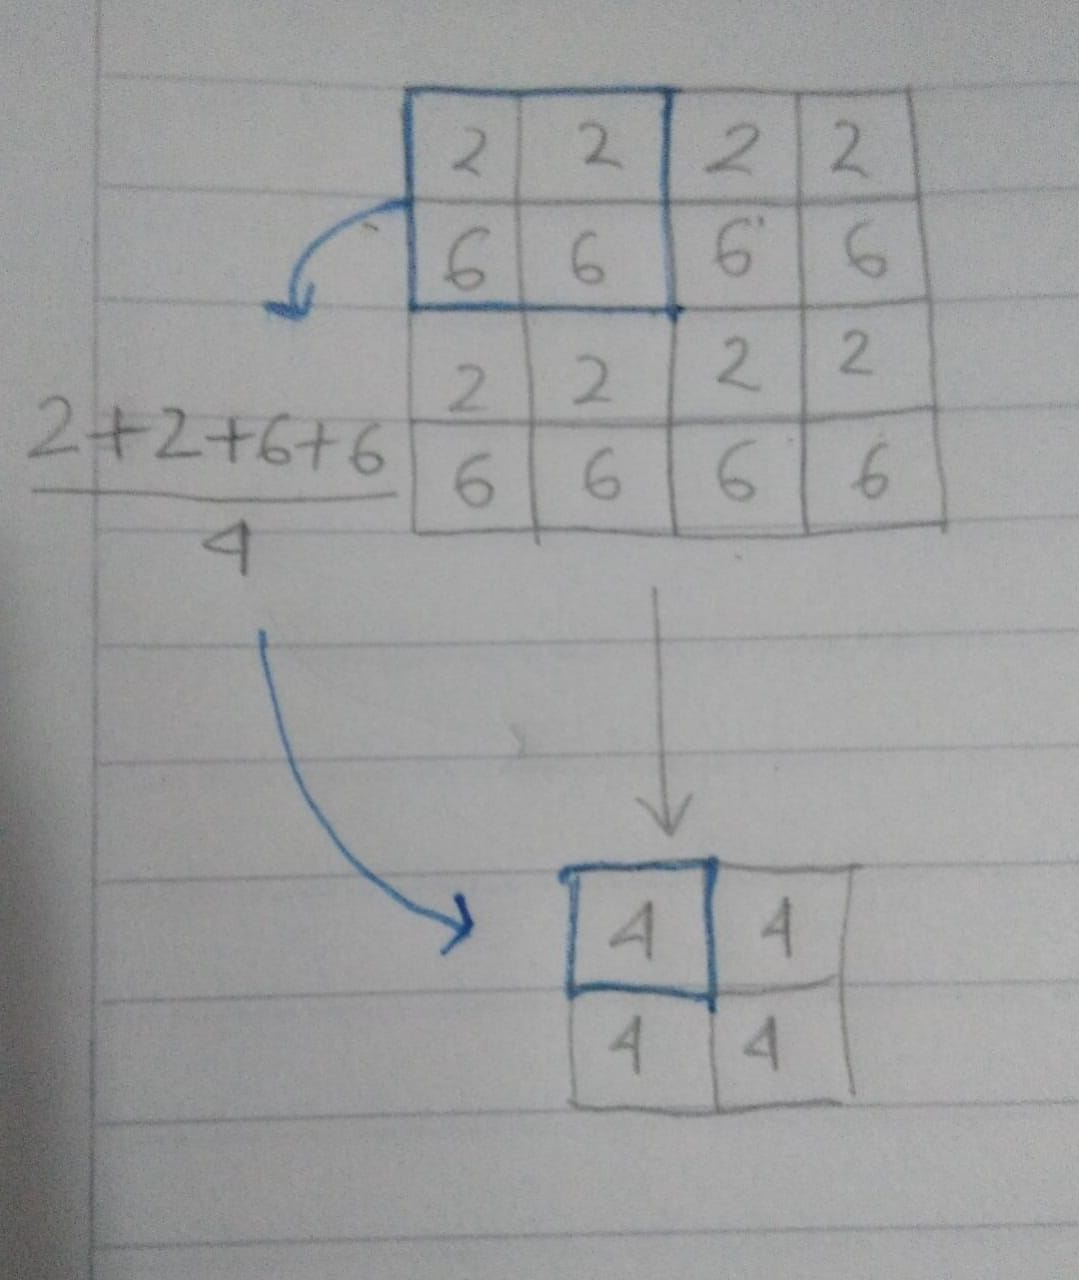
\includegraphics[width=8 cm]{Image.jpeg}
\centering
\caption{representacion visual algoritmo}
\label{fig:Image}
\end{figure}

\subsection{Algoritmo de duplicado de pixeles}

También podemos considerar el siguiente algoritmo:\\

Por medio de este algoritmo se duplicaran los pixeles brindando así que se mantenga una estructura de la imagen y no pierda su forma, aunque no será perfecta, será una alternativa para desarrollar el problema(su representacion visual se puede ver en figura 4).

\begin{figure}[h]
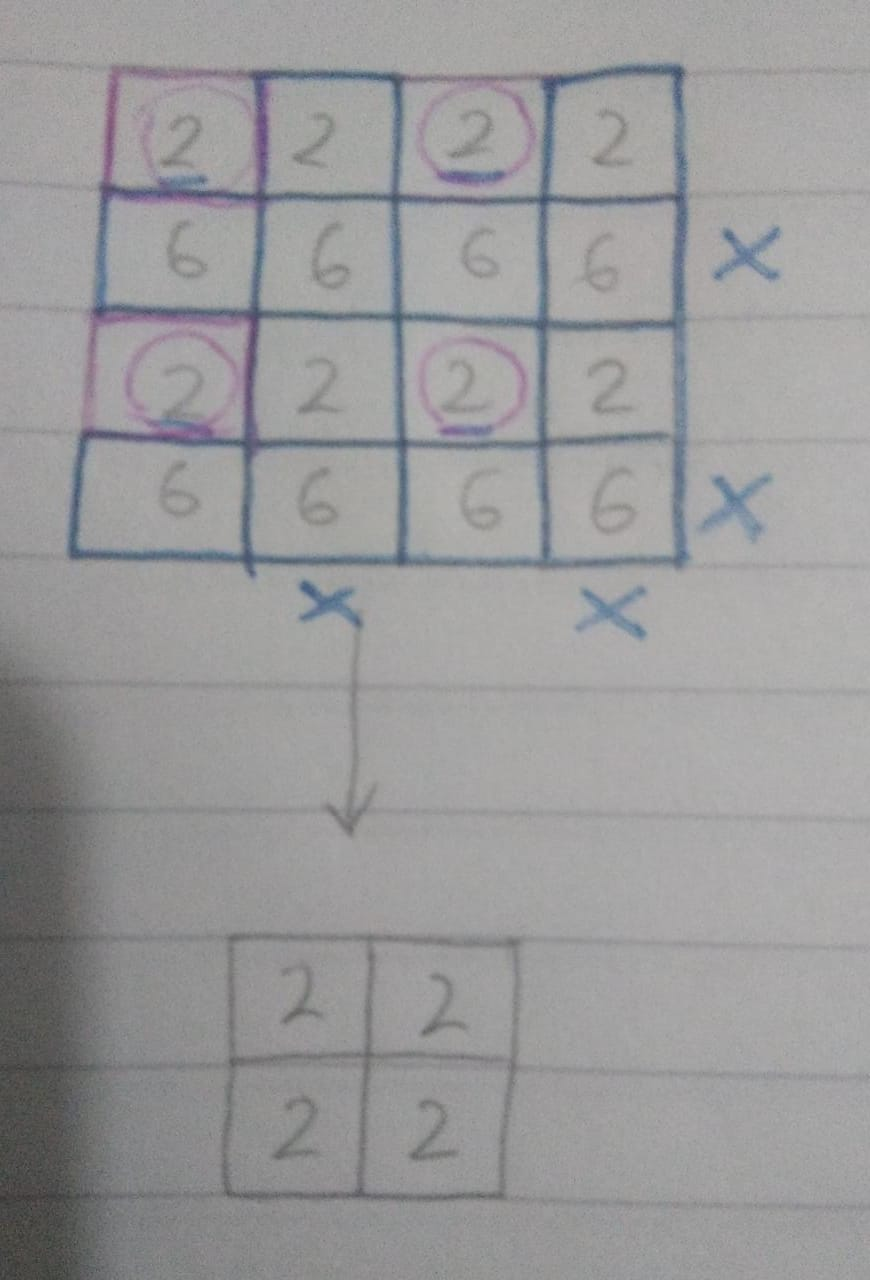
\includegraphics[width=8 cm]{Image_2.jpeg}
\centering
\caption{representacion visual algoritmo 2}
\label{fig:Image_2}
\end{figure}

\section{Consideraciones a tener en cuenta}

--los algoritmos pueden tener cambios en su estructura.\\

--Hacer copias de tinkercad para evitar algunas de las problematicas de la plataforma.\\

--Si es necesario se podran crear mas clases.\\


\end{document}